\begin{figure}

	\begin{subfigure}{0.49\columnwidth}
		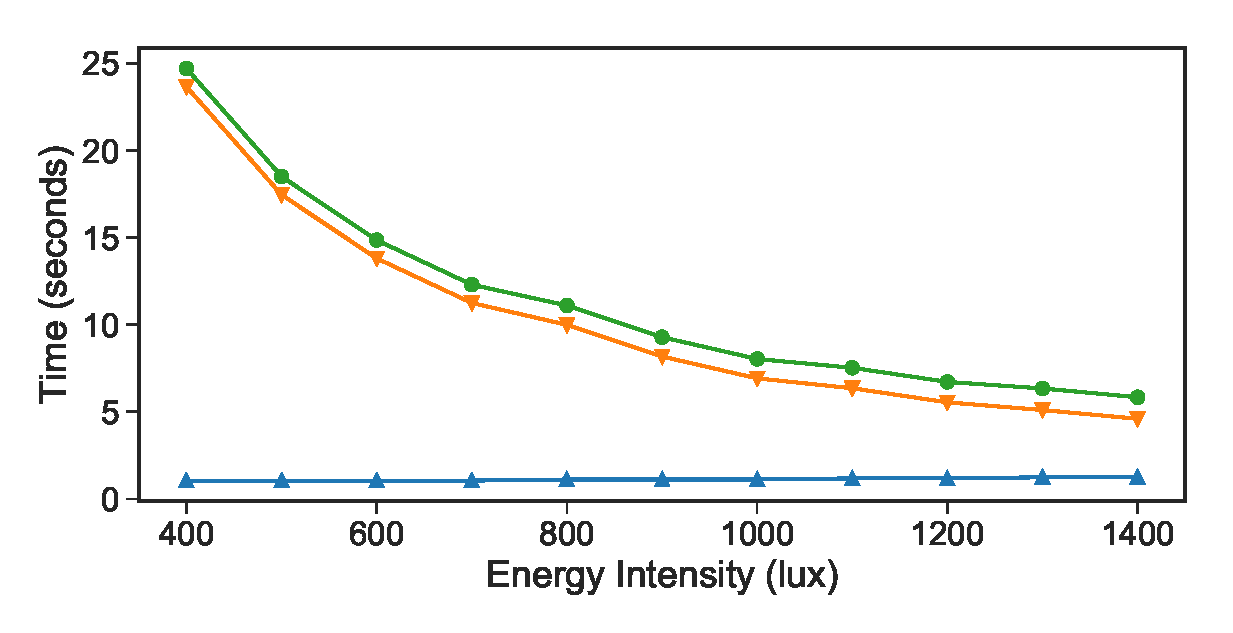
\includegraphics[width=\textwidth]{figures/BatterylessNodesDutyCycles_Active_mode}
		\caption{The node powers up and goes into active mode. The high energy consumption rate at this mode makes the changes in the on-time due to changes in ambient energy very small. }
	\end{subfigure}\hfill
	%
	\begin{subfigure}{0.49\columnwidth}
		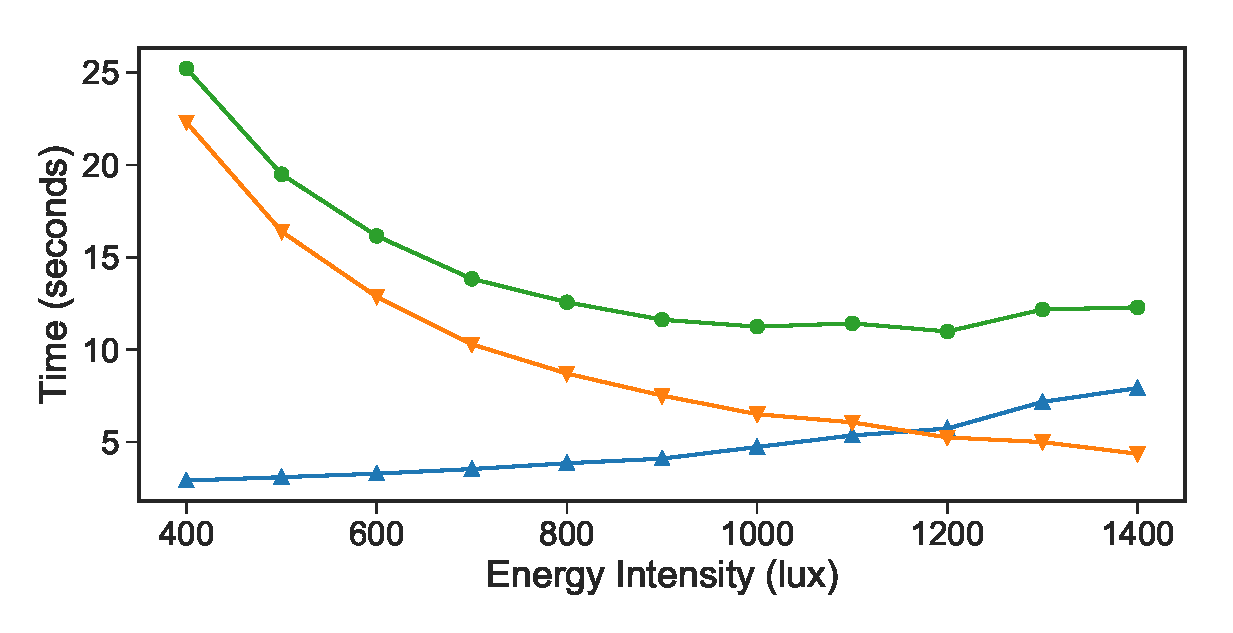
\includegraphics[width=\textwidth]{figures/BatterylessNodesDutyCycles_Sleep_mode}
		\caption{The node powers up and goes into sleep mode. The low energy consumption rate at this mode makes the changes in the on-time when ambient energy changes clearly noticeable. }
	\end{subfigure}
	\caption{On-times, off-times, and power (charge-discharge) cycle of a batteryless energy-harvesting node.)}
	\label{fig:pwrCycleVSEnergyIntensity}
\end{figure}

\paragraph{Different energy harvesting rates}
It can happen that some of the nodes of a \cis be in the shadow while the rest is under direct sunlight (e.g., when curtains are being opened). 
As a consequence, nodes' power cycles will generally be significantly different (Figure~\ref{fig:pwrCycleVSEnergyIntensity} shows the on-times, off-times, and power cycles when the ambient energy ranges from 400 to 1400\,lux). Therefore, nodes will not be able to accurately estimate the collective availability of the system, which reduces the overall performance. 
Taking into consideration that energy density vary overtime (e.g., the shadow of a curtain moves as the relative position of the curtain to the sun changes), an averaging technique might mitigate the negative effect of non-uniform distribution of ambient energy. 

\paragraph{Using machine learning algorithms to improve intermittent sensing}
In the future we plan to dive deeper in studying partially captured data. 
Intermittent sensors may partially capture events. Classical recognition 
algorithms face difficulties dealing with partially captured data. 
Therefore, we want to investigate \emph{how much machine learning algorithms 
can improve the sensing quality of intermittent sensing?} 